\documentclass[a4paper,12pt]{article}
\usepackage{amsmath}
\usepackage{amssymb}
\usepackage[polish]{babel}
\usepackage{polski}
\usepackage[utf8]{inputenc}
\usepackage{indentfirst}
\usepackage{geometry}
\usepackage{array}
\usepackage[pdftex]{color,graphicx}
\usepackage{subfigure}
\usepackage{afterpage}
\usepackage{setspace}
\usepackage{color}
\usepackage{wrapfig}
\usepackage{listings}
\usepackage{datetime}

\renewcommand{\onehalfspacing}{\setstretch{1.6}}

\geometry{tmargin=2.5cm,bmargin=2.5cm,lmargin=2.5cm,rmargin=2.5cm}
\setlength{\parindent}{1cm}
\setlength{\parskip}{0mm}

\newenvironment{lista}{
\begin{itemize}
  \setlength{\itemsep}{1pt}
  \setlength{\parskip}{0pt}
  \setlength{\parsep}{0pt}
}{\end{itemize}}

\newcommand{\linia}{\rule{\linewidth}{0.4mm}}

\definecolor{lbcolor}{rgb}{0.95,0.95,0.95}
\lstset{
    backgroundcolor=\color{lbcolor},
    tabsize=4,
  language=C++,
  captionpos=b,
  tabsize=3,
  frame=lines,
  numbers=left,
  numberstyle=\tiny,
  numbersep=5pt,
  breaklines=true,
  showstringspaces=false,
  basicstyle=\footnotesize,
  identifierstyle=\color{magenta},
  keywordstyle=\color[rgb]{0,0,1},
  commentstyle=\color{blue},
  stringstyle=\color{red}
  }

\begin{document}

\noindent
\begin{tabular}{|c|p{11cm}|c|} \hline 
Grupa 4 & Barbara Nowak, Piotr Tomaszewski & \ddmmyyyydate\formatdate{06}{11}{2016} \tabularnewline
\hline 
\end{tabular}


\section*{Zadanie 2 - Mnożenie macierzy MPI}

Celem naszego zadania było zaimplementowanie programu, którego zadaniem jest obliczenie iloczyn dwóch macierzy kwadratowych wypełnionych liczbami losowymi wg wzorów podanych w specyfikacji zadania oraz zastosowanie standardu MPI.



Program uruchamiany jest z argumentami: \quotedblbase size \textquotedblright - to liczba procesów (pobierany przy kompilacji za pomocą parametru -n )  a \quotedblbase rozmiarMac \textquotedblright- to rozmiar macierzy. Pierwszym etapem jest sprawdzenie poprawności podanego rozmiaru macierzy. Podobnie jak w zadaniu 1, deklarujemy potrzebne zmienne oraz macierze, alokujemy pamięć dla macierzy oraz uzupełniamy je wartościami wg wskazanych wzorów.
Na tym etapie rozpoczyna się nasza praca ze standardem MPI, który wymaga zainicjowania następujących funkcji, niezbędnych do dalszych obliczeń:

\begin{lstlisting}
	MPI_Init (&argc, &argv);               				//  inicjuje obliczenia MPI  (pierwsza funkcja MPI)
	MPI_Status status;    				   				//  okreslenie zrodla i typu komunikatu
 	MPI_Comm_rank (MPI_COMM_WORLD, &nr_procesu); 		//  komunikator, podanie numeru procesu
 	MPI_Comm_size (MPI_COMM_WORLD, &dostepne_procesy);  //  komunikator, podanie liczby procesorow
\end{lstlisting}

Kolejnym krokiem, jest podzielenie macierzy w taki sposób aby każdy proces obliczał wskazany mu fargment, a nie zajmował się niepotrzebnie obliczaniem całej macierzy. Ma to na celu przyśpieszenie obliczeń rozwiązywanego zadania.
Zadaniem poniższych funkcji jest wysłanie komunikatów (rozmiarWiersza i rozmiarStart) o długości równej 1 ( typu LONG) od procesu docelowego 0 za pomocą komunikatora MPI-COMM-WORLD.
\begin{lstlisting}
	MPI_Send(&rozmiarWiersza, 1, MPI_LONG, id_zadania, 0, MPI_COMM_WORLD);	
	MPI_Send(&rozmiarStart, 1, MPI_LONG, id_zadania, 0, MPI_COMM_WORLD);
\end{lstlisting}
Następnie dokonujemy synchronizacji wszystkich procesów w grupie, za pomocą poniższej funkcji MPI-Barrier i rozpoczynamy pomiaru czasu obliczeń z pomocą MPI-Wtime().
\begin{lstlisting}
	MPI_Barrier(MPI_COMM_WORLD);
\end{lstlisting}

W następnym etapie używamy funkcji, odpowiedzialnych za odbiór i odczytanie komunikatów, które zawierają dane o tej samej długości i typie jak w funkcji Send, jednak w tym przypadkiem źródłem nadanego komunikatu jest proces o randze 0, który zawiera wszystkie procesy MPI-COMM-WORLD. Znacznik MPI-ANY-TAG informuje, że typ wiadomości nie będzie sprawdzany.
\begin{lstlisting}
	MPI_Recv(&rozmiarWiersza, 1, MPI_LONG, 0, MPI_ANY_TAG, MPI_COMM_WORLD, &status);		
	MPI_Recv(&rozmiarStart, 1, MPI_LONG, 0, MPI_ANY_TAG, MPI_COMM_WORLD, &status);
\end{lstlisting}
Teraz musimy wykonać operację sumowania , gdzie wynik jest zwracany do jednego procesora(roota) za pomocą funkcji MPI-Reduce oraz ponowną synchronizację wszystkich procesów w grupie. Kończymy pomiar czasu obliczeń oraz implementujemy końcową instrukcję, jaką musi wykonać program korzystający z MPI - MPI Finalize() kończącą pracę programu.


\begin{wrapfigure}{r}{0.5\textwidth}
	\vspace{-40pt}
	\begin{center}
		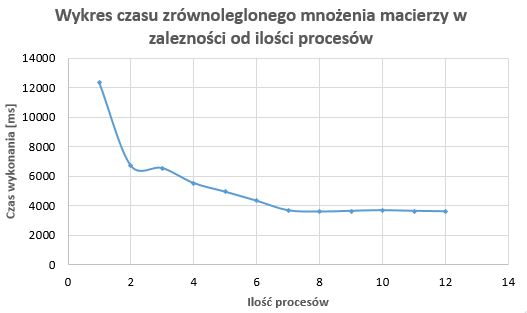
\includegraphics[width=0.5\textwidth]{img1.jpg}
	\end{center}
	\vspace{-20pt}
	\caption{Wykres zależności czasów od liczby procesów}
	\vspace{25pt}
\end{wrapfigure}

Do celów ćwiczeniowych, nasze macierze przyjeliśmy o rozmiarze \textit{1000x1000}. Wykres przyspieszenia zrównoleglonego mnożenia macierzy w zalezności od ilości procesów (Rysunek 1) dla mnożenia macierzy A i B, ukazuje, że wraz ze wzrostem liczby procesów czas obliczeń również się zwiększa. Przy pięciu procesach czas znacznie się zwiększa i drastycznie opada, by znów znacznie się zwiększyć pczy ośmiu procesach po których płynnie opada aż do osiągnięcia stabilnego poziomu. 



\begin{wrapfigure}{r}{0.5\textwidth}
	\vspace{-40pt}
	\begin{center}
		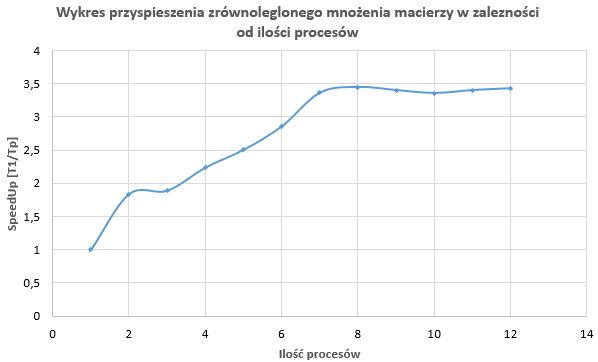
\includegraphics[width=0.5\textwidth]{img2.jpg}
	\end{center}
	\vspace{-20pt}
	\caption{Wykres przyspieszenia}
	\vspace{35pt}
\end{wrapfigure}


Proces zrównoleglenia przy pomocy MPI również bardzo dobrze obrazuje poniższy wykres czasu zrównoleglonego mnożenia macierzy w zalezności od ilości procesów (Rysunek 2). Widzimy tutaj, że program zwalnia aż do osiągnięcia ośmiu wątków a następnie zrównolegla się. 

\textbf{Podsumowanie:} MPI (ang. Message Passing Interface) to interfejs przesyłania komunikatów pozwalający na współdzielenie kodu przez wiele proocesów. Każdy z procesów zajmuje się przydzielonymi mu obliczeniami. MPI cechuje uniwersalność, ponieważ może być stosowany na wielu platformach, zrozumiałość gdyż równoległość i komunikacja są jawne. Jest również mobilny, pozwala na przenoszenie programu, a także wygodny, pozwala na zrównoleglenie programu na czym nam głównie zależało. W porównaniu do technologii OpenMP, która działa na wątkach, to MPI na początku jest trudniejsze w zrozumieniu i implementacji. W OpenMP nie musieliśmy zwracać uwagi jak dzielimy dane oraz co i jak przesyłamy między procesami. OpenMP wykonywał wszystko za nas, działając na wątkach. 


\end{document}
